% Write the full path to the location of the graphics relative to book.tex
\graphicspath{{chapters/chp1/graphics/}}

\title{Function scaling and boundary condition throttling for convergence control in highly nonlinear Poisson-Boltzmann electrolyte models.}
\titlerunning{Function Scaling and Convergence Throttling}

\author{D.~F.~Parsons, M.~Farci,  A.~Grigoras, Dagmawi Tadesse}
\authorrunning{Parsons et al.}

\institute{D.~F.~Parsons \email{drew.parsons@unica.it}
  \and M.~Farci \and A.~Grigoras
  \at University of Cagliari,
Department of Chemical and Geological Sciences \& CSGI,
Cittadella Universitaria, S.S. 554 bivio Sestu,
09042 Monserrato (CA), Italy
\and Dagmawi Tadesse
\at Murdoch University,
Discipline of Physics, Chemistry and Mathematics, 90 South St, Murdoch 6150, West Australia
}

\maketitle

\abstract{ The nonlinear Poisson-Boltzmann model of electrolyte
  solutions combines the Poisson equation for electrostatic potentials
  with a Boltzmann equilibrium of mobile ion concentrations. The
  Boltzmann equation $c = c_0 \exp[-e\psi/kT]$ is highly
  nonlinear once the electrostatic potential exceeds several thermal
  energy ($kT$) units (i.e.\ when $\psi>0.1$ V). This introduces two
  related numerical challenges. Firstly, suitable convergence conditions
  for the concentration functions become sensitive to the
  boundary potential. Secondly a controlled initial guess must be
  provided must be provided to avoid the FEM calculation diverging to
  NaN. We resolve the first challenge by logarithmic scaling of the
  concentration function, as suggested by the exponential nature of
  the Boltzmann equation.  However a nontrivial complex logarithmic
  form (``log-zero scaling'') is required in order to allow for the near-zero concentrations
  of coions. The second challenge is resolved  with an adaptive
  throttling algorithm that suppresses large
  boundary conditions down to the linear regime, then iteratively
  applies the throttled solution as an initial guess until the
  nonlinear solution  is iteratively  obtained.
  Our implementation
  allows for other nonelectrostatic molecular interactions important
  for modelling real chemical and electrochemical systems, in
  particular steric forces due to finite ions sizes, enabling
  computation of concentrated electrolytes with electrode potentials
  as high as 2000V. We provide a general derivation of the weak and
  strong forms of the system from the underlying thermodynamic energy functional. }

\section*{Introduction}

Continuum theory (mean field theory) has been an effective tool for
studying the behaviour of systems in electrolyte solutions. The
Poisson-Boltzmann (PB) model \cite{Wu2022} enables evaluation of ion
adsorption layers at surfaces together with the electric field that
surface charge and adsorbed ions generate. The PB model underpins
theory of stability of microparticle suspensions in aqueous media,
enabling modelling of particle aggregation and surface forces. The
same theory can also be applied to model electrochemical
systems, including energy storage devices, batteries or
supercapacitors. But there is a crucial difference in the two classes
of application, which has a significant impact on the numerical
stability of the model.  The surface potentials
of typical microparticles such as protein molecules or metal oxide
particles tends to lie in the range 5--50 mV, which is 0.2--2
$kT$ in thermal energy units (based on a thermal potential at $T=298$
K defined by $e\psi_{T} = kT$, where $e$ is the elementary charge, $k$
is Boltzmann's constant, $T$ is temperature). Electrolytic energy
storage systems, by contrast, typically operate with electrode
potentials of the order of 1--5 V, that is 1000--5000 mV, or 40--200
$kT$.  The nonlinearity of the Poisson-Boltzmann model is highly
sensitive to energies exceeding one $kT$ unit, requiring particular
algorithms to enable numerical nonlinear convergence.  Our goal is to
set up the calculation to solve successfully over a broad range of
electrode potentials without requiring manual readjustment of
convergence parameters.  We identify two main steps, implemented via
finite element methods (using FEniCSx\cite{baratta2023dolfinx}): log-scaling of
ion concentration functions, and throttling of boundary
conditions. For context we also present a summary of the physics and
weak formulation defining the Poisson-Boltzmann model, including
finite ion size effects.
In order to focus on the numerical algorithms, we omit redox
phenomenon (including electrolysis of water) which would occur in real
systems at such high electrode potentials.

\section{Weak formulation of the Poisson-Boltzmann model}

The energy functional for an electrolyte solution, determined by
electrostatic potential $\psi(x)$ and ion concentration profiles
$c_i(x)$, may be composed from various fundamental energy
contributions as
\begin{equation}
    \Omega[\psi, c_i] = \Omega_{el} + \Omega_{en} +  \Omega_{ex}
\end{equation}
$\Omega_{el}$ describes the direct energy of the electrostatic field generated by the electric charge of ions and surfaces, \cite{Jackson_Classical_Electrodynamics}
\begin{equation}
  \Omega_{el}  =\frac{1}{2} \int_{V}D \cdot E dx
  = -\frac{1}{2} \int_{V}D \cdot E dx + \sum_i \int_V z_i e c_i(x) \psi(x) dx
  + \int_{S} \sigma(s) \psi(s) ds
\end{equation}
where $E$ is the electric field, $E=-\nabla\psi$, and $D$ is the
electric displacement $D=\varepsilon_0
\varepsilon(x)E$. $\varepsilon_0$ is the permittivity of the vacuum,
and $\varepsilon(x)$ is the (spatially varying) relative
permittivity. $z_i$ is the valency of ion $i$.  $\sigma(s)$ is the
surface charge density on boundary $S$.

$\Omega_{en}$ describes the ideal entropic energy of ions, treated as ideal (noninteracting) particles \cite{GrayStiles2018,DagmawiParsons2024},
\begin{equation}
    \Omega_{en} = kT \sum_{i} \int_{V} \left[ c_i(x) \ln \left(\frac{c_i(x)}{c_{i\infty}} \right) - c_{i}(x) + c_{i\infty} \right] dx 
\end{equation}
where $c_{i\infty}$ is the bulk concentration of ions. As a point of
physics, it is important to note that the use of a fixed bulk
concentration means the system is controlled by the chemical potential
of ions, with a variable number of ions in the domain $V$ of interest.
That is, the thermodynamic potential is a grand potential, not a
(Helmholtz) free energy, and for that reason we write the energy as $\Omega$ rather
than $F$. A free energy formulation (with fixed number of ions) would
require use of a thermal de Broglie wavelength instead of
$c_{i\infty}$ \cite{GrayStiles2018}.

$\Omega_{el} + \Omega_{en}$ alone construct the conventional
Poisson-Boltzmann model. The term $\Omega_{ex}$ represents extra
contributions to the total energy functional that describe other
relevant physics, such as pH-dependent charge regulation
\cite{ParsonsSalis2019}, specific ion interactions
\cite{ParsonsCarucciSalis2022}, or steric forces due to finite ion
size \cite{LopezGarciaHornoGrosse2018}. We consider the latter in this
work.

The Poisson-Boltzmann model describes the system in equilibrium,
obtained by minimising the total grand potential with variation
$\delta\Omega=0$ with respect to $\psi$ and $c_i$. Variation with
respect to $\psi$ (with test function $p \equiv \delta \psi$) leads to a weak formulation
for the Poisson equation,
\begin{equation}
    0 = -\int_{V} \varepsilon_{0}\varepsilon(x) (\nabla\psi,\nabla p) dx + \sum_{i}z_i e \int_{V} c_{i}(x) p dx + \int_{S} \sigma(s) p ds  
    \label{weak_Poisson}
\end{equation}
for all test functions $p$ in the relevant finite element space.  After additional
integration by parts, this weak formulation leads to the strong
formulation of the electrostatic Poisson equation,
$\nabla\cdot D = \sum_i z_i e c_{i}(x)$.

The variation of $\Omega$ with
respect to each ion concentration profile $c_i$ (in turn, with test
functions $b_i\equiv \delta c_i$), assuming linear variations such that
$\ln(1+b_i/c_i)\approx b_i/c_i$, leads to the weak formulation of Boltzmann's
equation,
\begin{equation}
    0 = \int_{V} \left[ e z_i \psi(x)
    + kT \ln\left(\frac{c_i(x)}{c_{i\infty}}\right)
  \right] b_i dx
    \label{weak_Boltzmann}
\end{equation}
for all test functions $b_i$. The strong form of the classical Boltzmann equation can then obtained, $c_i(x)=c_{i\infty}\exp(-z_i e \psi(x)/kT)$. 

It might be noted that in the classical Poisson-Boltzmann model, the
ion concentrations $c_i$ are determined completely by the
electrostatic potential with the Boltzmann equation in closed form, so
only the Poisson equation would need to be solved directly. However, the
physical problem with the classical model is evident in electrochemical
systems with electrode potential 1 V. A one volt potential is
equivalent to a thermal energy of $40 kT)$, for which the conventional
Boltzmann factor for a counterion is
$\exp(40)\approx 2.3 \times 10^{17}$.  That is, the surface counterion
concentration of a 1M electrolyte would exceed $10^{17}$ mol/L, which
is clearly unphysical.  We return the model back to physical
relevance by adding an extra steric energy term $\Omega_{ex}$ with
corresponding excess chemical potential per ion $\mu_{i}^{ex}$, for
which the modified Boltzmann equation is
\begin{equation}
    c_i(x)=c_{i\infty}\exp\left[(-(z_i e \psi(x) + \mu_i^{ex}(x)-\mu_{i\infty}^{ex})/kT\right]
    \label{general_Boltzmann}
\end{equation}
This corresponds to a total chemical potential $\mu_i(x)$ of each ion,
defined by
\begin{eqnarray}
  \mu_i(x) &=& \mu_{i}^{\textrm{entropic}} +  \mu_{i}^{\textrm{electrostatic}} +
               \mu_{i}^{ex} \\
{} &  =&\mu_{i\infty} + kT \ln(c_i(x)/c_{i\infty})
         + ez_i \psi(x) + \mu_i^{ex}(x)-\mu_{i\infty}^{ex}.
         \label{chem_pot}
\end{eqnarray}
$\mu_{i\infty}$ refers to the (fixed) excess chemical potential of the
ion in bulk solution, defined relative to an ideal unit
reference solution by $\mu_{i\infty} = kT\ln c_{i\infty} + \mu_{i\infty}^{ex}$.
The steric model we employ is the Carnahan-Starling model
\cite{CarnahanStarling1969} with a contribution to the grand potential
% for future reference, the CS model (both energy and chemical
% potential)  can be considered as Padé approximations
% i.e. rational  polynomials functions
% which give good convergence when used in the Homotopy Series Method
% thus tells us Liao
\begin{equation}
    \Omega_{ex} = \sum_{i} \int_{V} c_{i}(x) \left[ kT
    \frac{4\phi - 3\phi^2}{(1-\phi)^2}
    -  \mu_{i\infty}^{ex}
  \right]dx
  \label{CS_energy_functional}
\end{equation}
and weak formulation
\begin{equation}
    0 = \int_{V} (\mu_i^{ex}-\mu_{i\infty}^{ex}) b_i
    \label{weak_CS}
\end{equation}
for all $b_i$, which adds to \eqnref{weak_Boltzmann}, the weak
formulation for the Boltzmann equation, together generating the strong
formulation of the modified Boltzmann
equation,  \eqnref{general_Boltzmann}.  Here the excess chemical potential
per ion for the Carnahan-Starling model, corresponding to the energy
functional \eqnref{CS_energy_functional}, is
\begin{equation}
    \mu_{i}^{ex} = kT \frac{\phi(8-9\phi+3\phi^2)}{(1-\phi)^3}
    \label{chem_pot_CS}
\end{equation}
$\phi$ is the \emph{total} ion volume fraction defined by
$\phi=\sum_i c_i v_i$ where $v_i$ is the intrinsic molar volume per
ion $i$. Hence the CS excess chemical potential is defined identically
for all ions. To derive the weak formulation in \eqnref{weak_CS}, we
applied an homogenised component approximation that assigns common
volumes at the point of introducing the variation  $\delta c_i$ (which
is the test function $b_i$), such that $\delta\phi=v_j \delta c_i$ rather
than $v_i \delta c_i$. This approximation is required since the CS
model was formulated for single component systems. The more complex
multicomponent BMCSL model would enable ion specific chemical
potentials \cite{MansooriCarnahanStarlingLeland1971}, removing the
need for this approximation.  $\phi_{\infty}$, $\mu_{i\infty}^{ex}$
are the bulk total volume fraction and excess chemical potential
defined by bulk concentrations $c_{i\infty}$. With this term, the
Boltzmann equation \eqnref{general_Boltzmann} becomes transcendental in $c_i$, precluding a closed
expression that would determine ion concentrations. Concentration functions must therefore be
explicitly solved  numerically alongside potential $\psi$. In this
paper we address strategies for managing the strong nonlinearity in
the system introduced by this term when large values of the
potential are present. Note that $c_i$ must also be solved explicitly in the case
of time-dependent nonequilibrium Poisson-Nernst-Planck (drift-diffusion) systems \cite{LopezGarciaHornoGrosse2018} where
ion concentrations are not in equilibrium and determined by a
continuity equation rather than a Boltzmann equation.

One last point on the weak formulation of the Boltzmann equation. The variational
derivation of these weak formulations from the energy functionals,
\eqnref{weak_Boltzmann} and \eqnref{weak_CS}, presents them in terms of the
chemical potential of the ions, \eqnref{chem_pot}, not the concentration directly. That
is, fundamentally the strong form of the Boltzmann equation is simply $\mu_i(x) =
\mu_{i\infty}$, the condition of equal chemical potential at all
points in the domain in equilibrium with an external bulk bath.
The Boltzmann
equation in terms of 
concentration, \eqnref{general_Boltzmann}, is then simply a rearrangement of
the strong equation for chemical potential. Since chemists are in the
habit of using the Boltzmann equation in concentration form rather
than chemical potential, in practice our implementation in code applies the weak
form of the Boltzmann equation via concentrations, as
\begin{equation}
0 =   \int_V \left[ c_i(x) - c_{i\infty}
    e^{-\left(z_i e \psi(x) +
      \mu_i^{ex}(x)-\mu_{i\infty}^{ex}\right)/kT} \right] b_i
dx 
\label{weak_Boltzmann_conc}
\end{equation}
for all test functions $b_i$, rather than applying it via the chemical
potential components in \eqnref{weak_Boltzmann}
+\eqnref{weak_CS}. Because the concentration functions $c_i(x)$ being
solved are the same, this change in weak form should not affect
residuals. The question can be asked, though out of scope
to answer here, whether these alternative weak forms for the Boltzmann
equation affect efficiency, perhaps by changing the condition number
of the matrices used to solve the Poisson-Boltzmann system. Our
testing found the chemical potential formulation to be less stable than the
concentration formulation (failing to converge with an 1V electrode
potential, where the latter weak form achieves successful convergence
with the log-zero concentration scaling described next).

\section{Nonlinear mesh}
The nonlinear solution requires a finer mesh in the nonlinear region
close to an electrode boundary, rendering solutions on a uniform linear mesh  impractical at electrode
potentials greater than 0.1V.  The general exponential nature of the potential,
$\psi(x) \sim \psi_{0} \exp(-\kappa x)$, suggests logarithmic spacing of
mesh may be suitable. The strongly nonlinear  system
considered here  would be a good candidate for adaptive mesh refinement. In
lieu of adaptive remeshing, however, we find a sufficient nonlinear
mesh spacing can be achieved with a geometric sequence of mesh points,
multiplying the points $x$ of a uniform unit interval by $x^3$ to
obtain finer spacing for the points closer to the boundary at $x=0$.

\section{Function scaling}
We constructed a finite element implementation of the weak
formulation (\eqnref{weak_Poisson} and \eqref{weak_Boltzmann_conc}) in
FEniCS-X \cite{baratta2023dolfinx}, using continuous 
Lagrange elements with polynomial order 2 (linear elements with order
1 may also be used).  The electrolyte solution
is taken as NaCl with bulk concentration 1 mol/L.  To illustrate
general issues of nonlinear convergence, we calculate the
electrostatic and ion concentration profiles of ion adsorbed at a
single flat electrode surface along the direction perpendicular to the
surface, with the electrode boundary at $x=0$.  The electrode
potential is controlled (Dirichlet boundary condition), and bulk
solution represented by a zero Neumann condition (``zero electric
field'') at  a distance of 30 Debye lengths (at $x=9.1$ nm, for the 1M
electrolyte). Nonlinear solutions are computed using FEniCS-X's
NonlinearProblem with a standard NewtonSolver. Convergence criterion
is set to dolfinx's default ``incremental'' method with absolute
tolerance $10^{-5}$.
We set PETSc options \cite{PETSc_manual,petsc4py_2011} configuring the solver to use the LU direct
solver provided by MUMPS \cite{MUMPS_2001,MUMPS_2019}, with the PETSc Krylov type set to apply the
preconditioner only once (\verb|ksp_type=preonly|, \verb|pc_type=lu|,  \verb|pc_factor_mat_solver_type=mumps|).
By contrast, for instance, a
conjugate gradient solver (\verb|ksp_type=cg|, \verb|pc_type=gamg|)
generates a spurious oscillatory electrostatic potential profile with electrode
potentials higher than 0.1 V.

The electrostatic potential $\psi(x)$ is handled with trivial
scaling, solving $P(x)=\psi(x)/\psi_0$, where $\psi_0$ is the
electrode potential.
But we must take more care scaling the concentration functions
$c_i(x)$.
We already noted that the counterion concentration becomes unphysically
large in the conventional Poisson-Boltzmann model due to nonlinear
exponentiation of  electrostatic potentials exceeding 0.1--0.2 V in
the Boltzmann equation. Trivial scaling may be introduced by solving
the concentration function scaled against the bulk concentration. But
 the nonlinear catastrophe is reached
numerically above 0.5 V. Already at 0.6 V, the conventional
calculation with simple scaling is unable to reduce the residual below
the required convergence criterion  $10^{-5}$. While it would be possible to relax the
convergence tolerance to obtain a reasonable solution, our aim is to
obtain a robust general solver not requiring close manipulation of
convergence criteria. For instance,  modelling the
cyclic voltammetry curve of an electrode may require calculations
over a potential window as wide as $-5$ to 5 V.

The challenge arises due to the extreme magnitudes of the counterion
concentration at the electrode surface. The weak formulation for the
Boltzmann equation in \eqnref{weak_Boltzmann} suggests a solution:
solve for the concentration function in log-form,
\begin{equation}
C_{i}(x) = \ln[ c_{i}(x) / c_{i\infty}]
\label{log_scaling}
\end{equation}
rather than the physical concentration function $c_{i}(x)$ directly. Log
scaling extends the solvability of the conventional point-charge Poisson-Boltzmann
model up to electrode potentials as high as 1.5 V. Solutions for the
electrostatic potential and counterion concentration profile are shown
in \figref{fig_classical_PB}. Shown on a log scale, strong
nonlinearity in the PB system becomes apparent in the bend in the
electrostatic potential (\figref{fig_classical_PB}a) close to the
surface where $x<2$\AA\ for electrode potentials $> 0.2$ V.


\begin{figure}
\centering
(a)
\includegraphics[width=0.45\linewidth]{counterion_potential.eps}
(b)
\includegraphics[width=0.45\linewidth]{counterion_logzero.eps}
\caption{\label{fig_classical_PB}Solutions to the classical point
  charge Poisson-Boltzmann model of 1M NaCl electrolyte solution,
  shown as profiles along $x$, the perpendicular distance from an
  electrode surface (a) Electrostatic potential. (b) Counterion
  (\ce{Cl-}) concentration. }
\end{figure}

At still higher potentials the stability of simple log scaling with
respect to the coion must be considered. The coion, with same charge
as the electrostatic potential, is repelled from the electrode surface,
resulting in coion concentrations trending towards zero near the electrode. At
sufficiently high potentials this generates values in the log-scaled
function that tend towards $-\infty$, which destabilises the numerical
solution (residuals become infinite). We therefore introduce a more complex log-scaling function,
\begin{equation}
Z_i(x) = \ln\left[c_i(x)/c_{i\infty}+1\right]/\ln 2 - 1
\label{log_zero}
\end{equation}
which keeps the scaled coion function constrained between -1 and 0
rather than $-\infty$ and 0. Since this scaling function addresses the
near-zero concentration of the coion, we call it ``log-zero'' scaling.

\section{Throttling algorithm}

Log-scaling of concentration functions facilitates a successful numerical solution to
the conventional Poisson-Boltzmann at electrode potentials
up to 1.5V. Nevertheless \figref{fig_classical_PB}b demonstrates the
point charge catastrophe of the conventional model, with counterion
concentrations exceeding $10^{5}$ mol/L at the electrode
surface. Moreover, for general electrochemical applications it would
be desirable to be capable of obtaining solutions for electrode
potentials higher than 1.5V. To deal with the physical problem, we
introduce finite ion sizes with a steric force provided by the
Carnahan-Starling model, \eqnref{chem_pot_CS} (weak form
\eqnref{weak_CS}).  We apply ion volumes
$v_{\ce{Na}}=1.24 \textrm{\AA}^{3}$ per \ce{Na+} ion,
$v_{\ce{Cl}}=35.9 \textrm{\AA}^{3}$ per \ce{Cl-} ion (volumes taken from
quantum mechanical volumes of the ions' electron clouds
\cite{ParsonsNinham2009}).

The additional nonlinearity introduced by the Carnahan-Starling model,
where the chemical potential depends on the concentrations being
calculated, introduces a new challenge. The default nonlinear solver
in FEniCS assumes zero as an initial guess for the functions being
solved. But under the nonlinear conditions (with electrode potential
$>0.2$ V) where the Carnahan-Starling steric force is required, the
zero initial guess leads quickly to a diverging solution with infinite
or NaN
residual. And yet a stable solution is accessible at lower values of
the boundary condition. We nudge the solver to a stable solution by
applying a throttling algorithm: reduce the boundary condition to a
small value for which a solution can be obtained, then incrementally
increase the boundary value back towards the target value, using the
previous found solution as an initial guess for the next
iteration. The approach is known to mathematicians as a homotopy
method \cite{homotopy_analysis_Liao2012}
or numerical continuation method \cite{allgower1990numerical},
with our throttle serving as a homotopy parameter applied to boundary
conditions.  A flowchart for the algorithm is shown in
\figref{fig:throttling_algorithm}.

\begin{figure}
\centering
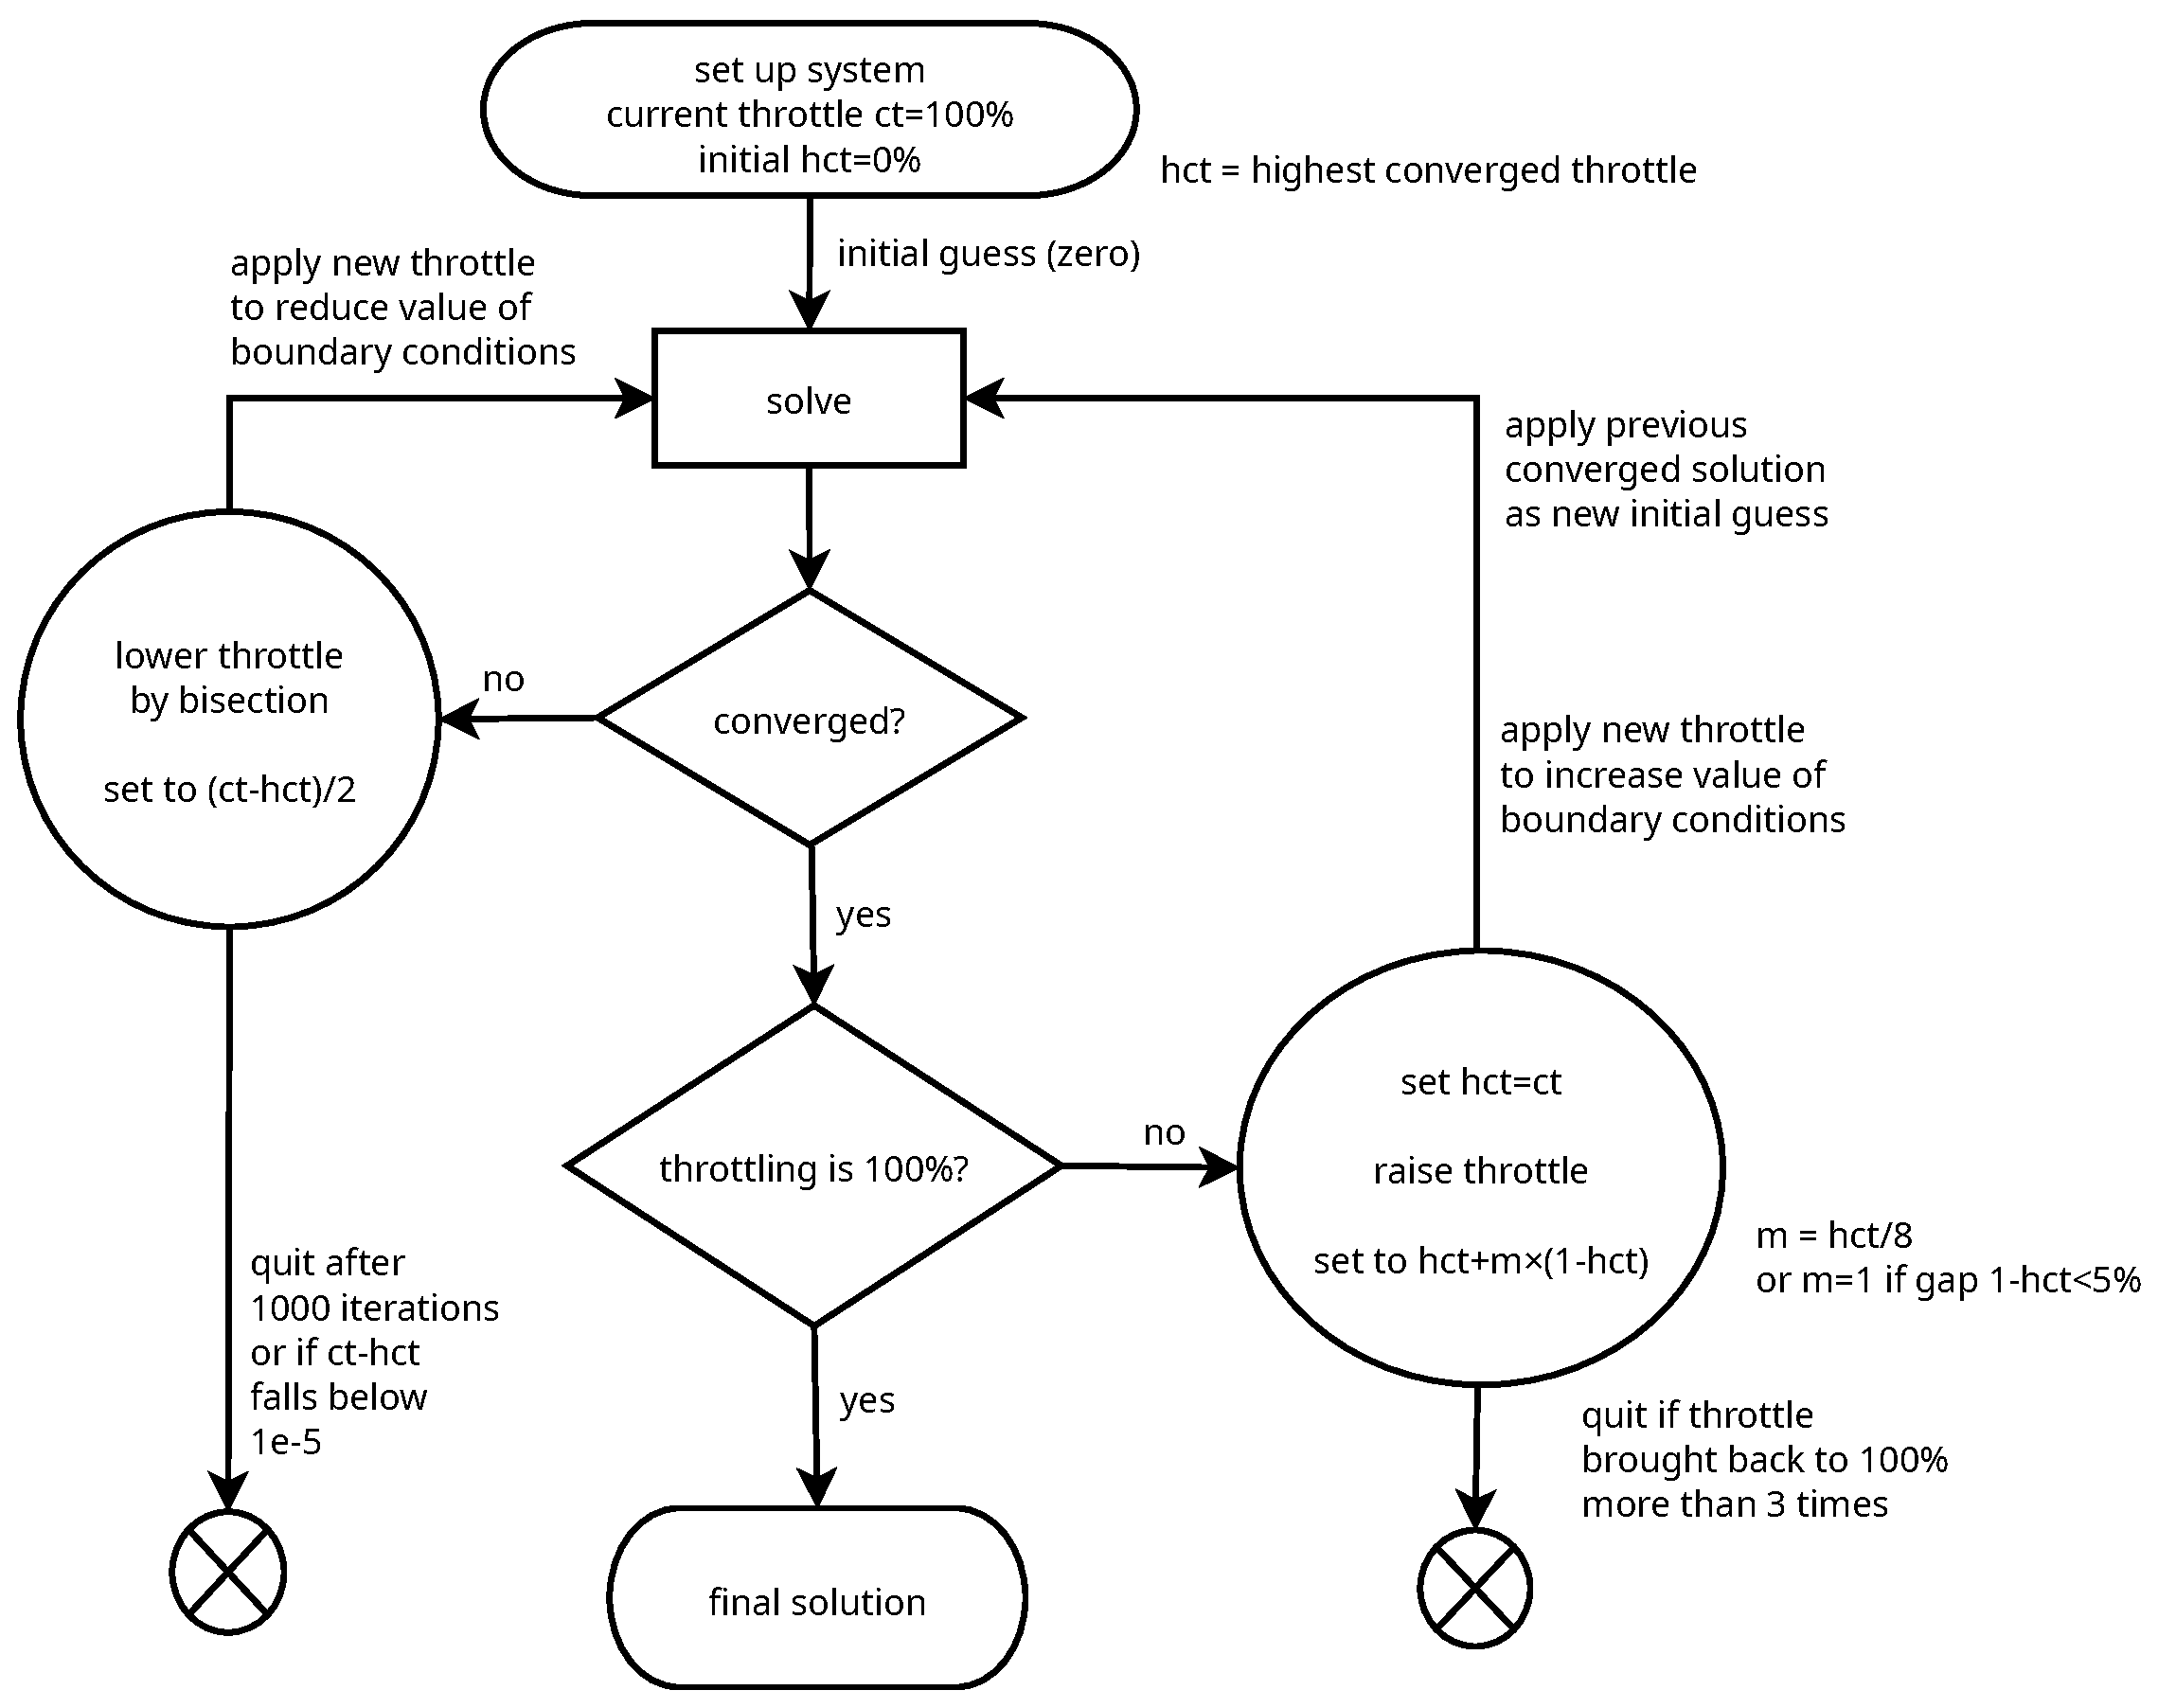
\includegraphics[width=0.8\linewidth]{throttling2.eps}
\caption{Flowchart for the throttling algorithm. }
\label{fig:throttling_algorithm}
\end{figure}

The throttle is a multiplier
applied to the magnitude of the boundary conditions.
If the solver fails to converge, then reduce the throttle downwards by
bisection between the current failed value (``current throttle'', ct) and the highest converged
throttle (hct, initially 0). Once the boundary
condition is throttled low enough to generate a converged solution,
update the hct and raise
the throttle upwards by an amount $u$, towards 100\% (set the throttle
to 100\% if the procedure would exceed it).  The value of $u$
must find a balance between reaching 100\% throttle in as few
iterations as possible (don't make $u$ too small), while not collapsing back to non-converging
conditions when raising the throttle (don't make $u$ too
large). Empirically we find that when the hct is small, the rise rate
must also be small to obtain the next converged iteration. Once hct is
large, the rise rate may be proportionally larger. We therefore
propose a rise rate $u=m\times \mathrm{hct}$, such that the next
throttle applied after a converged iteration is
\begin{equation}
  \mathrm{ct [new]} = \mathrm{hct} + m (1-\mathrm{hct})
\end{equation}
with
\begin{equation}
  r=
  \begin{dcases}
    \frac{\mathrm{hct}}{r} & \\
    1 & \text{if } 1-\mathrm{hct} < 5\%
  \end{dcases}
\end{equation}
This produces a quadratically accelerating rise rate (and attempts a
direct jump to 100\% once the remaining gap is less than 5\%).  It is likely
that our formulation, quadratic in hct, approximates a more 
optimal exponential (or
sigmoidal) rise rate.
An example of
the  throttle rate against number of iterations is shown in
\figref{fig:throttle_rate} for 1V and 10V boundaries with different
choices of fixed values of $r$. A best value of $r$ can be identified
for each voltage, minimising the number of iterations required,
e.g. $r=2$ for 1V, and $r=3$ for 10V. A
value of $r$ larger than the best value means the rise rate is
smaller, such that convergence is smooth, but requires more
iterations. A lower value of $r$ means the rise step is too large,
overstepping and resulting in a nonconverging iteration, such that
more iterations are required to fall back to a converging throttle rate.

\begin{figure}
\centering
(a)
\includegraphics[width=0.45\linewidth]{test_1V.eps}
(b)
\includegraphics[width=0.45\linewidth]{test_10V.eps}
\caption{Attempted throttle rate vs iteration number, for (a) 1V and
  (b) 10V  boundaries with fixed rise rate multipliers $r=1,2,3$ and 4.
}
\label{fig:throttle_rate}
\end{figure}

The best-performing fixed values of $r$  for potentials up to 1000V are shown
in  \figref{fig:best_throttle_rate}. The trend suggests empirically that an
optimal multiplier follows
$r \propto \ln V$, indicating that $r$ 
may be tuned adaptively to provide the maximum possible rise rate (smallest
possible $r$) that minimises the number of unsuccessful non-converged
attempts for the given boundary condition.  A milder
rise rate (larger $r$) is required at larger surface potentials.
Allowing for a finite value of $r$ when $V \rightarrow 0$, we propose
an adaptive definition of $r$,
\begin{equation}
  r(V) = 1 + A \ln(1 + B V)
  \label{adaptive_r}
\end{equation}
This model imposes the limit $r \rightarrow 1$ as $V \rightarrow 0$.
In principle an optimal low-voltage multiplier might take $r<1$, if
$r>$hct, but the limit 1 is simpler, avoiding the need to 
compare against hct.  Fitting against best $r$ for log-zero scaling
obtains $A=1.3$ and $B=0.7 \textrm{V}^{-1}$. Best $r$ for trivial
scaling is similar to log-zero scaling.
We emphasise that the value of $V$ used in the adaptive $r$ formula, \eqnref{adaptive_r},
must be the target boundary condition (the final electrode voltage),
not the throttled boundary condition at the given iteration.  If a throttled $V$ were
applied, $r$ would be small when the boundary condition is strongly
throttled, resulting in large rise steps that cause convergence
failure when the  target voltage is large.


\begin{figure}
\centering
\includegraphics[width=0.8\linewidth]{best_r_vs_v.eps}
\caption{Best fixed rate multiplier $r$ for each voltage, giving lowest
  number of throttling iterations.
}
\label{fig:best_throttle_rate}
\end{figure}



Table.~\ref{tab:convergence} shows  the number of iterations required
to converge with various boundary conditions for the different
concentration scaling functions, in both the point charge model and the
steric model, and applying adaptive
$r(V)=1+1.3\ln(1+0.7V)$. For the point charge model, trivial scaling only
permits calculation up to 0.5V. Log scaling reaches 1.3V, log-zero
scaling reaches 1.9V.

\begin{table}
  \centering
  \begin{tabular}{c|ccc|ccc}
pot(V)  & \multicolumn{3}{c|}{Point charge} & \multicolumn{3}{c}{Steric}    \\
        & trivial & log & log-zero & trivial & log & log-zero \\ \hline
%%%%%%%%%%%%%%%%%%%%%%%%%%%%%%%%%%%%%%%%%%%%%%%%%%%%%%%%%%%%%%%%%%%%%%
%%                                                                  %%
%%  This is a LaTeX2e table fragment exported from Gnumeric.        %%
%%                                                                  %%
%%%%%%%%%%%%%%%%%%%%%%%%%%%%%%%%%%%%%%%%%%%%%%%%%%%%%%%%%%%%%%%%%%%%%%
%NaCl 1M	&	&	&	&	&	&\\
%	&pot(x)/surf\_pot + non linear geometry 	&	&	&	&	&\\
%	&Steric OFF	&Steric OFF + log	&Steric OFF + log\_zero	&Steric ON	&Steric ON + log	&Steric ON + log\_zero\\
%Surface Potential [V]	&Throttle attemps	&	&	&	&	&\\
0.1	&1	&1	&1	&1	&1	&1\\
%0.2	&1	&1	&1	&1	&6	&6\\
%0.3	&1	&1	&1	&1	&9	&9\\
0.5	&1	&1	&1	&1	&12	&9\\
0.6	&F	&1	&1	&1	&12	&12\\
1	&	&1	&1	&1	&16	&13\\
1.3	&	&55	&41	&8	&17	&17\\
1.4	&	&S	&143	&8	&17	&17\\
%1.5	&	&S	&187	&8	&17	&18\\
1.9	&	&	&573	&9	&21	&18\\
2	&	&	&S	&9	&22	&18\\
%3	&	&	&	&14	&23	&23\\
5	&	&	&	&20	&30	&30\\
10	&	&	&	&27	&F	&39\\
%25	&	&	&	&56	&	&52\\
%50	&	&	&	&92	&	&72\\
100	&	&	&	&132	&	&122\\
%250	&	&	&	&240	&	&180\\
%375	&	&	&	&355	&	&212\\
%500	&	&	&	&419	&	&230\\
%625	&	&	&	&478	&	&321\\
%750	&	&	&	&517	&	&382\\
%875	&	&	&	&551	&	&428\\
1000	&	&	&	&586	&	&463    \\
2000	&	&	&	&S	&	&647    
  \end{tabular}
\caption{\label{tab:convergence}Number of throttling iterations
  required to  solve the  Poisson-Boltzmann model of a 1M NaCl electrolyte solution
  for various electrode potentials and concentration scaling
  functions (trivial, log, or log-zero scaling), for both the classic point charge model, and the steric
  model (Carnahan-Starling) with finite ion sizes. Adaptive rise rate
  multiplier $r(V)=1+1.3\ln(1+0.7V)$.
  ``F''=Failed
  (throttle step $<10^{-5}$). ``S''=Stopped at 1000 iterations.}
\end{table}


The corresponding
performance plot of iterations vs voltage for the steric model
(trivial and log-zero scaling) is shown in \figref{fig:convergence}
Trivial scaling is successful with the steric model up to 1000V, while simple log
scaling fails at 10V due to instability introduced by near-zero coion
concentrations.
Log-zero scaling enables calculation to 2000V
and greater, beyond the limit of trivial scaling. But the steric model
naturally keeps concentrations within 
physically reasonable bounds, such that  log-zero scaling is not
required for normal electrochemical conditions. In fact
trivial scaling performs better than log-zero scaling when $V<20$V,
the region of electrochemical interest.
But even with log-zero scaling, computation of the interaction of
100~kV electrical transmission cables with saline water would require
such a large number of iterations that this algorithm would become impractical.

\begin{figure}
\centering
\includegraphics[width=0.8\linewidth]{a_v_V.eps}
\caption{Number of throttling iterations,  as a function of electrode
  voltage, needed to solve the steric model with trivial and log-zero scaling.
  Applies an adaptive rise rate multiplier $r(V)=1+1.3\ln(1+0.7V)$.
}
\label{fig:convergence}
\end{figure}

These final performance tests used adaptive $r$ coefficients taken from log-zero scaling ($A=1.3$,
$B=0.7 \textrm{ V}^{-1}$). One could fit against the best fixed  $r$ for trivial
scaling (to get $A=1.2$, $B=1.4 \textrm{ V}^{-1}$), but empirically
the performance overall is (marginally) better with the log-zero
parameters, even when applied to calculations using trivial scaling.




Samples results of the adaptive throttling algorithm for an electrode charged to
10V, with Carnahan-Starling steric forces, are shown in
\figref{fig_results_throttling}, calculated with trivial scaling of the
concentration functions. \figref{fig_results_throttling}b shows the onset
of a steric adsorption layer \cite{DagmawiParsons2022} with counterion
concentrations constrained below a concentration cap determined by the
ion size (a cap of 46 mol/L in the case of our \ce{Cl-} ion).

\begin{figure}
\centering
(a)
\includegraphics[width=0.45\linewidth]{steric_potential_10V.eps}
(b)
\includegraphics[width=0.45\linewidth]{steric_10V_counterion.eps}
\caption{\label{fig_results_throttling}Solutions to the modified
  Poisson-Boltzmann model of a 1M NaCl electrolyte solution with
  Carnahan-Starling steric forces, shown as profiles along $x$, the
  perpendicular distance from a 10V electrode surface (a) Electrostatic
  potential. (b) Counterion (\ce{Cl-}) concentration. }
\end{figure}

\section{Conclusion}

Modelling complex electrolyte solutions in electrochemical conditions
with electrode potentials 1V or greater requires both nontrivial
physics and nontrivial numerical algorithms.
With respect to the
physics, aside from redox chemistry and electrolysis (not considered
here), the finite sizes of ions must be taken into consideration via
steric forces. These are expressed as a steric contribution to the
chemical potential of ions and used in the underlying thermodynamic
energy functional that provides the origin of both the weak and strong
formulations of the system.
In order to achieve numerical convergence, we have proposed two
steps. Firstly, we propose log-zero function scaling of
concentration functions that accounts
not only for the heightened concentrations of counterions near an
electrode, but also the near-zero concentrations of coions. Secondly,
we propose a throttling algorithm (a kind of homotopy method) that reduces boundary conditions
down to the linear regime where a solution is easily obtained, then
progressively propagates that solution by releasing the throttle
until the target boundary condition is obtained. Optimised convergence
is obtained by adaptively controlling the rise rate of the throttle factor
depending on the target boundary condition.

The combination of
log-zero scaling and throttling facilitates calculations of point
charge models up to 2V. Log-zero scaling enables
the steric model to reach electrode potentials greater than 2000V.
But for typical electrochemical applications with potentials lower than 20V,
where steric forces are needed in order to maintain the physical relevance
of the model, trivial scaling is sufficient and indeed faster than log-zero scaling.
We illustrated the throttling algorithm using Dirichlet boundary
conditions (electrode potentials), but the  principle applies
equally to Neumann or more complex boundary conditions.

\begin{acknowledgement}
  We acknowledge the award of CINECA support under the ISCRA
  initiative, for the availability of high-performance computing
  resources and support.
\end{acknowledgement}

\bibliographystyle{spbasic}
% Write the full path of your bibfile relative to book.tex
\bibliography{chapters/chp1/bibliography.bib}


